\documentclass{scrartcl}
\usepackage[ngerman]{babel}
\usepackage[utf8]{inputenc}
\usepackage{booktabs}
\usepackage{graphicx}
\usepackage{hyperref}
\bibliographystyle{plain}

\begin{document}
\title{Dokumentation Projektarbeit - GameOfLife}
\author{Groth, Frederick}
\date{\today}
\maketitle
\newpage
\tableofcontents
\newpage
\section{Einleitung}
Das Game of Life wurde 1970 vom Mathematiker J.H. Conway entwickelt. Es ist ein zellulärer Automat, welcher nach deterministischen Regeln funktioniert.

Sowohl räumlich, als auch zeitlich ist dieser diskret aufgebaut. Es wird ein zweidimensionales Feld betrachtet, welches lebende oder auch einfach besetzte und tote oder auch leere Zellen enthält. In diskreten Zeitschritten wird anhand der Nachbarzellen und des Zustandes der Zelle selbst bestimmt, ob sie auch im nächsten Zeitschritt lebend bleibt oder neu geboren wird.

Die Regel, die dies bestimmt, lautet im Standartbeispiel B3/S23, das bedeutet, eine Zelle wird bei 3 lebenden Nachbarzellen geboren ('\textbf{b}orn'). Bereits lebende Zellen überleben ('\textbf{s}urvive') bei 2 oder 3 lebenden Nachbarzellen.
\section{Ziel des Projektes}
Ziel des Projektes war die Programmierung des GameOfLife in Python.
Dies bedeutet, dass an Hand einer vom Benutzer vorgegebenen Regel die Entwicklung des Feldes berechnet und dargestellt werden soll. Ferner wurden einige Sonderfunktionen programmiert, welche dem Benutzer weitere Einstellungen ermöglichen.
\section{Vorüberlegungen}
Zunächst habe ich mir überlegt, wie ich mein Programm aufbauen will. Eine Strukturierung in verschiedene Funktionen, welche ineinander eingebunden werden, erschien mir am sinnvollsten. Die Vorgabe der Parameter sollte über Text-Dateien geregelt werden, wofür ich ebenfalls eine vorbereitende Funktion erstellen wollte.

Nun blieb nur noch zu klären, wie ich das Feld mit den Zellen darstellen sollte. Es bestand die Möglichkeit, nur die lebenden Zellen als Koordinatenpaare zu speichern, wobei meiner Meinung nach die Abfrage der Nachbarn eher kompliziert gewesen wäre. So entschied ich mich dafür, alle Zellen als Matrix zu speichern, mit 1en für lebende und 0en für tote Zellen. Bei dieser Variante sind die vorhanden Funktionen von Numpy sehr hilfreich.
\section{Durchführung}
Das Projekt wurde in mehrere Arbeitsschritte eingeteilt. Zunächst wurde GitHub als Versionskontrollsystem eingerichtet, um das Projekt zu sichern und den Verlauf zu dokumentieren. Anschließend begann die Programmierarbeit mit dem Erstellen der Grundfunktionen, die für das Programm nötig sind. Ich entschied mich dafür, die Strukturen von Numpy zu verwenden, insbesondere also arrays und den zugehörigen Operationen zu arbeiten. Die genaue Funktionsweise ist dem Programm und insbesondere den Funktionsbeschreibungen zu entnehmen. Hier soll nur ein kleiner Einblick in die generellen Strukturen und zugehörigen Überlegungen gegeben werden.

Die folgende Reihenfolge gibt vor allem einen logisch sortierten Überblick. Bei der Programmierung selbst wurden Programmfehler teilweise erst später behoben, während schon mit anderen Funktionen begonnen wurde, oder Einstellungen wie die Randbedingung erst später ins Programm ergänzt.
\subsection{prepGoL}
Ein wichtiger Aspekt des Programms sollte die Vorgabe einiger Bedingungen vom Nutzer sein. Dazu zählen der Regelstring, welcher den Verlauf bestimmt, die Randbedingung, Systemgröße, sowie die Anfangsbedingung. Zu diesem Zweck schrieb ich die Funktion prepGoL. Diese verlangt genau diese Eigenschaften als Argumente, welche in verschiedenen Formaten vorgegeben werden. Die erste Idee war, alle Argumente in eine Text-Datei zu schreiben. Dies wäre allerdings beim Datenimport deutlich komplizierter gewesen, da die verschiedenen Argumente verschiedene Variablen-Typen benötigen. Die Funktion prepGoL erstellt also mehrere Text-Dateien, welche noch einmal verändert werden können. Jede Datei enthält ein Argument. Die Dateien werden zum Ausführen der Funktion GameOfLife in genau der vorgegeben Form benötigt.
\subsection{GoLdataimport}
Zur weiteren Verwendung müssen die Daten wieder als Variablen importiert werden. Dies geschieht mit der Funktion GoLdataimport, welche eine Null-Matrix der vorgegebenen Größe erzeugt. Sie wird an den in der Anfangsbedingung vorgegebenen Stellen mit 1en gefüllt. Diese stehen im weiteren Verlauf für lebende Zellen, 0en für tote/nicht vorhandene Zellen. Das nun fertige Anfangsfeld wird gemeinsam mit der Randbedingung zurückgegeben.
\subsection{GoLStep}
Nun war also die Vorbereitung für den Import der Benutzervorgaben abgeschlossen. Ich habe mich anschließend der Berechnung der folgenden Matrix zugewandt. Dazu muss zunächst einmal die Anzahl der Nachbarzellen jeder Zelle berechnet werden. Da ich mich, wie schon erwähnt, für die Arbeit mit Matrizen, genauer numpy arrays, entschieden hatte, bot sich hierfür eine Matrixmultiplikation (M.dot(M1)) an. Nach näher Betrachtung ergab sich, dass die Multiplikation mit Matrizen mit 1en auf der Hauptdiagonale sowie den beiden nächsten Nebendiagonalen das gewünschte Ergebnis lieferte. Auf der linken Seite  erwirkt dies eine Addition der untereinander liegenden Werte, auf der rechten Seite eine Addition der nebeneinander liegenden. Es muss schließlich noch die Feld-Matrix abgezogen werden, damit die Zellen selbst nicht mitgerechnet werden.

Somit lässt sich der Verlauf für eine begrenzte Randbedingung berechnen, bei der die Außenbereiche als tot angenommen werden. 

Später habe ich die Funktion für andere Randbedingungen ausgeweitet. Dazu gehören noch ein torusförmiges bzw. periodisches und ein unendliches Feld.
Für eine torusförmig gekrümmte Fläche, oder wie ich sie genannt habe, periodische, müssen in den beiden Matrizen noch 1en in den Ecken ergänzt werden.

Die Berechnung für eine unendliche Randbedingung gestaltet sich etwas schwieriger. Hier muss die Größe der Matrix dynamisch angepasst werden. Ich entschied mich dafür, die Matrix nur zu erweitern, nicht jedoch zu kürzen, falls in den Randbereichen keine lebenden Zellen sein sollten. Es wird also geprüft, ob sich in den Randbereichen lebende Zellen aufhalten. Dies geschieht ebenfalls mit Matrixmultiplikationen. 

Ist dies der Fall, wird eine weitere Zeile oder Spalte an der entsprechenden Seite ergänzt.

\subsection{GoLplot}
Da nun die Ausgangsmatrix sowie eine Funktion zum Berechnen der weiteren Schritte vorhanden war, habe ich mir überlegt, wie ich die Veränderungen animiert darstellen kann. Nach einer Suche auf den matplotlib Seiten stieß ich auf die Funktion FuncAnimation von matplotlib.animation. Diese erschien mir für meine Zwecke geeignet und so erarbeitete ich mir aus den Beispielen und der Dokumentation die Funktionsweise. Dies nutzte ich dann, um die Matrix animiert als imshow auszugeben. Als Parameter müssen dabei einerseits die Geschwindigkeit, Anzahl der Schritte, Wiederholungen und die Figur, in der geplottet wurde, übergeben werden. Andererseits wird eine Funktion benötigt, welche den Verlauf vorgibt. Dies gestaltete sich als schwerster Teil, da sie nur von der Schrittnummer abhängen darf und sie die Figur wieder zurückgeben muss.

Zunächst einmal musste gespeichert werden, wie die letzte  Matrix aussah. Um die Geschwindigkeit bei Wiederholungen zu erhöhen, werden alle Felder in einer Liste gespeichert und abgerufen. Sollte der Wert noch nicht in der Liste vorhanden sein, wird er aus dem vorhergehenden mit der Funktion GoLStep berechnet. Diese Listen und einige andere Werte wurden, um sie fehlerfrei in Unterfunktionen zu nutzen, auf global gesetzt.

Eine weitere Schwierigkeit trat auf, als ich die Darstellung aktualisieren wollte, wobei eine Veränderung der dargestellten Werte nicht ausreichte. Bei der unendlichen Randbedingung wird nur ein Ausschnitt der Anfangs-Größe angezeigt. Meine Lösung war schließlich die immer neue Erzeugung der imshow, nachdem der Darstellungsbereich geleert wurde.

Abschließend fügte ich noch eine wie i fortlaufende Variable hinzu, welche Pausen und Stopps möglich macht.

Die ebenfalls in der Funktion GoLplot vorhandenen Sonderfunktionen werden in einem späteren Abschnitt besprochen.

\subsection{GameOfLife}
Als Abschluss fügte ich noch die Funktion GameOfLife hinzu, welche, nach der Ausführung von prepGoL oder einem manuellen Erstellen der Text-Dateien, alle weiteren Funktionen aufruft und so den Ablauf vom GameOfLife ermöglicht.

Nach dem Datenimport werden die Variablen an GoLplot übergeben, sodass die Animation startet.

\section{Sonderfunktionen}
Zusätzlich zur rein animierten Ausgabe der Matrix habe ich noch einige Sonderfunktionen programmiert. Diese sind alle in GoLplot vorhanden, sodass sie neben der Matrix z.B. als Knöpfe dargestellt werden können.

Ich entschied mich, zunächst eine farbige Darstellung zu integrieren, später aber auch noch Start, Pause und Einzelschritts-Knöpfe zu erstellen. Ferner sollte eine Option zum Bearbeiten der Matrix und eine zum Erstellen einer neuen, leeren Matrix hinzugefügt werden.

Für all dies benutzte ich ipython widgets.
Anfangs versuchte ich noch, die Optionen im selben Fenster anzuzeigen. Aufgrund besserer Übersichtlichkeit verwendet das Programm nun eine Anzeige in einem neuen Fenster. Lediglich die Optionstasten zum Öffnen dieser Fenster, sowie die Start, Pause und Einzelschritt-Knöpfe sind im selben Fenster mit der Animation verblieben.

\subsection{Farbwahl}
Als erstes fügte ich eine Farbauswahl zur Funktion GoLplot hinzu, welche aus zwei Teilen besteht. Die erste Teilfunktion dient zur Farbwahl per Schalter, wobei verschiedene Farben gewählt werden können. Außerdem sind Schieberegler vorhanden, über welche die Farbe manuell eingestellt werden kann. Hierzu ist eine weitere Funktion vorhanden, welche aus der Farbwahl eine cmap erstellt und anwendet. Auch der Schalter benutzt diese Funktion, es wird je nach Farbwahl der Anteil an rot, grün und blau auf den Schiebereglern eingestellt und somit die entsprechende Funktion aufgerufen. Dies erkennt man in Abbildung (\ref{col})

\begin{figure}[!h]
	\begin{center}
		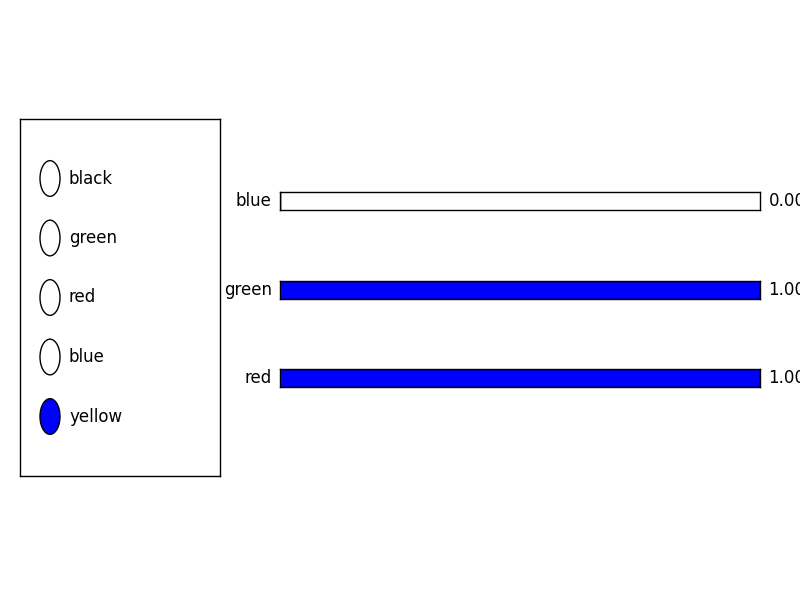
\includegraphics[width=\textwidth]{ColOpt.png}
		\caption{Aufbau der Farbwahl}
		\label{col}
	\end{center}
\end{figure}

\subsection{Manuelle Steuerung}
Für die manuelle Steuerung der Darstellung wurden vier Knöpfe erstellt, ein Pause-Knopf, ein Knopf für einen Einzelschritt nach vorne, ein Knopf für einen Einzelschritt zurück und ein Start-Knopf.

Um die Animation zu unterbrechen, wurde in die Funktion, welche den Verlauf bestimmt, eine Abfrage nach einer Bool-Variable pause hinzugefügt. Sollte pause wahr sein, so wird i konstant gehalten. Der Pause-Knopf setzt pause auf wahr, der Start-Knopf wiederum auf falsch. Zu diesem Zweck handelt es sich bei pause um eine globale Variable.

Außerdem wurde eine globale Variable für einen Einzelschritt in jede Richtung hinzugefügt, welche die Ausführung eines Schrittes erwirkt, hinterher aber wieder auf falsch gesetzt wird.

\subsection{Bearbeiten des Feldes}
Als weitere Funktion sollte dem Nutzer die Bearbeitung des Feldes per Maus-Klick ermöglicht werden. Dazu fügte ich einen Knopf hinzu, wobei die zugehörige Funktion nur ausgeführt wird, wenn die Variable editing auf wahr gesetzt wird, was gleichzeitig einen Stopp der Animation bewirkt.
Innerhalb der Funktion wird zunächst der Knopf auf die entsprechende Größe gesetzt. Ich habe entdeckt, dass die Höhe des Plot unverändert bleibt, wohingegen die Breite nach dem Verhältnis von Höhe zu Breite der Matrix variiert. Anschließend wird auf Attribute des Events zugegriffen. Somit lässt sich unter Berücksichtigung der Größe der Matrix die Koordinate berechnen, auf welche geklickt wurde.

An dieser Stelle wird der Wert der Matrix neu gesetzt, er errechnet sich aus dem Betrag von bisherigem Wert abzüglich eins, was aus einer Eins eine Null und umgekehrt macht.
Anschließend wird dies als neuer Anfangszustand gewählt.

\subsection{Grundeinstellungen}
Auch während des Programmablaufes soll dem Nutzer die Veränderung der Grundeinstellungen, wozu ich die Regel und die Randbedingung zähle, möglich sein. In einem neuen Fenster erscheinen sowohl ein Schalter zur Auswahl der Randbedingung, als auch insgesamt 18 Knöpfe zum Bearbeiten der Regel. Jeder dieser Knöpfe zeigt durch seine Farbe an, ob der Wert zur Regel gehört. Der Aufbau ist in Abbildung (\ref{gen}) zu erkennen.

\begin{figure}[!h]
	\begin{center}
		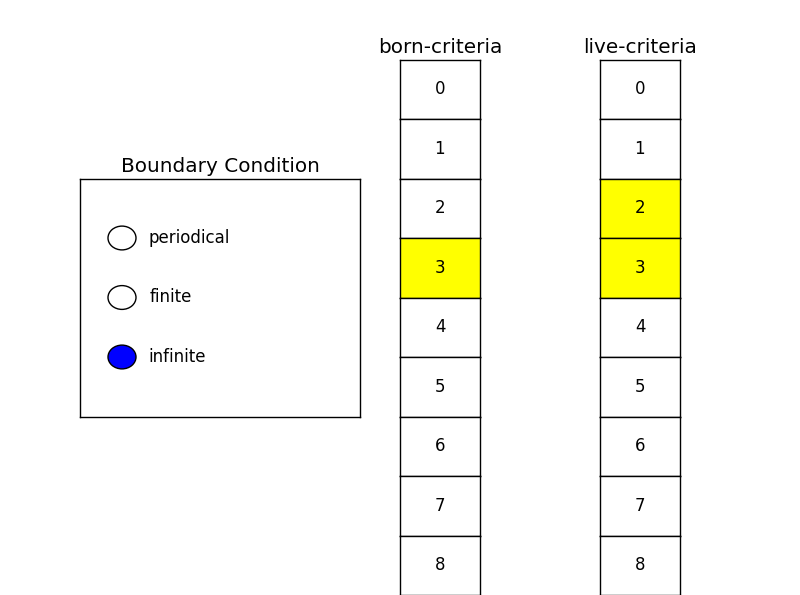
\includegraphics[width=\textwidth]{GenOpt.png}
		\caption{Aufbau der Grundeinstellungen}
		\label{blink1}
	\end{center}
\end{figure}

Um nicht 18-mal die gleichen Funktionen zu schreiben, fasste ich sie in einer Schleife zusammen, welche die Werte von Null bis Acht durchläuft, also alle mögliche Werte für die Regel. Zur eindeutigen Namenswahl wird dies in als String geschrieben, welcher durch den entsprechenden Wert ergänzt wird, und dann mit exec ausgeführt. Vor allem dazu waren die globalen Variablen nötig, um sie trotz der exec Umgebung abrufen zu können.
\subsection{Neues Feld}
Abschließend kann auch als letzte der Voreinstellungen die Feldgröße verändert werden. Dazu werden Knöpfe mit den entsprechenden Zahlen sowie ein Rückgängig- und ein Bestätigungsknopf erstellt. Damit kann zunächst die x-Größe, dann die y-Größe eingestellt werden, woraus ein neues leeres Feld der entsprechenden Größe erstellt wird. In der Abbildung (\ref{NewF}) ist eine solche Eingabe zu erkennen, bei der für die x-Größe bereits 12 eingegeben wurde, nach Drücken von Enter kann die y-Größe eingestellt, um dann mit Enter das neue Feld zu erstellen.
\begin{figure}[!h]
	\begin{center}
		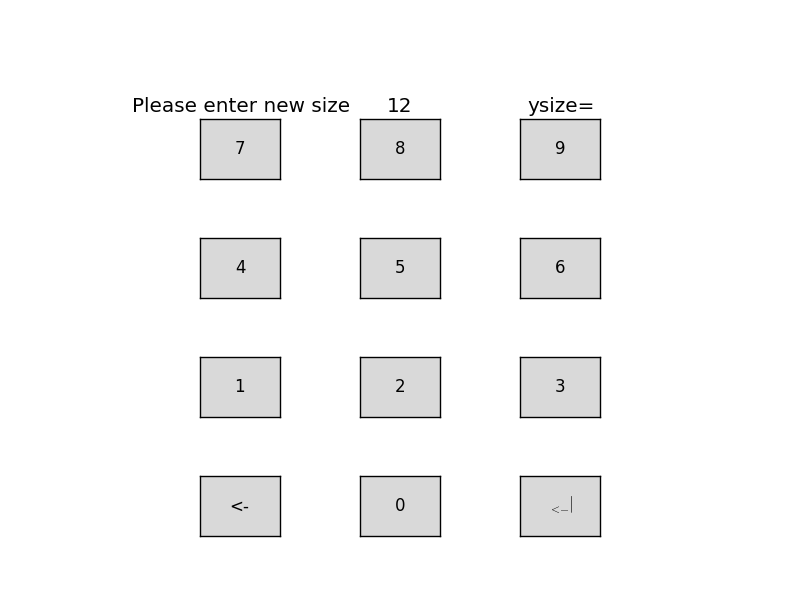
\includegraphics[width=\textwidth]{NewF.png}
		\caption{Neues Feld erstellen}
		\label{NewF}
	\end{center}
\end{figure}

\subsection{Beispiele}
Die Funktionen des Programms lassen sich einfach an der Ausgabe erkennen. Es gibt in bestimmten Welten Figuren, die sich periodisch verändern, statisch sind oder sogar fortbewegen.

Im Anhang sind einige dieser Beispiele zu finden. Sie wurden immer mit der Regel S23B3 durchgeführt. Setzt man die Startbedingung entsprechend der in den Dateien vorgegebenen Werte, entwickelt es sich entsprechend der Bilder.
\subsubsection{Blinker}
Der Blinker ist ein sich periodisch veränderndes Objekt, die Startbedingung der Animation ist unter dem Dateinamen \textit{GameOfLifeBlinker.dat} zu finden. Die Grafiken (\ref{blink1}) und (\ref{blink2}) wurde aufgenommen bei einer Feldgröße von 9*9 und einer periodischen Randbedingung.

Zu erkennen sind zwei solcher Blinker in beiden Zuständen.
\begin{figure}[p]
	\begin{center}
		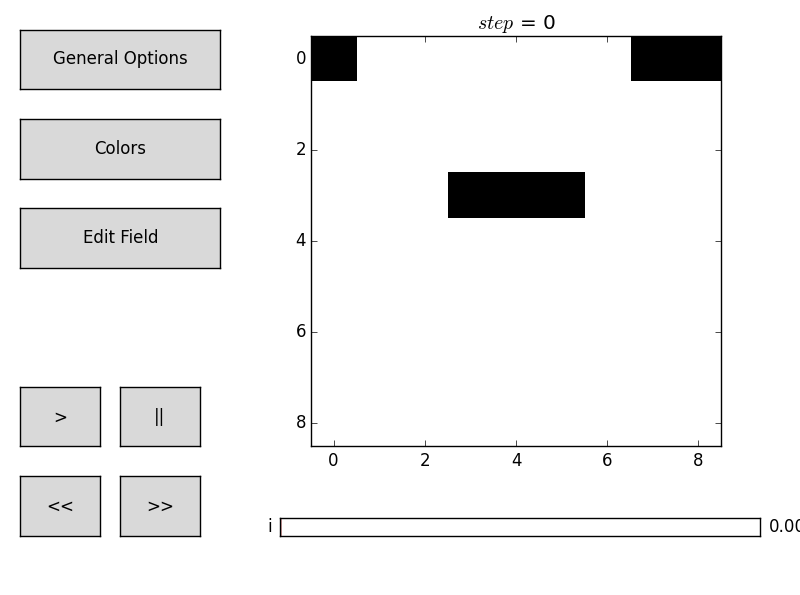
\includegraphics[width=\textwidth]{Blinker1.png}
		\caption{Zwei Blinker bei periodischer Randbedingung - Zustand 1}
		\label{blink1}
	\end{center}
\end{figure}
\begin{figure}[p]
	\begin{center}
		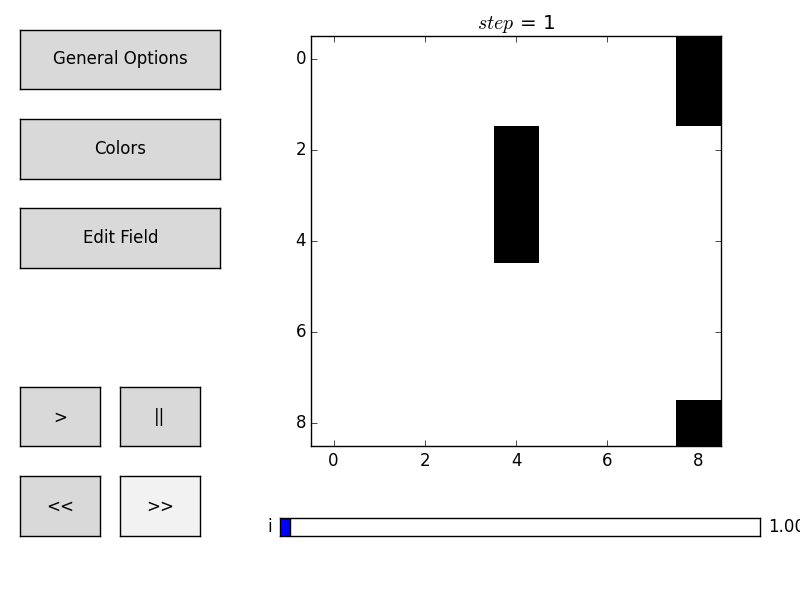
\includegraphics[width=\textwidth]{Blinker2.png}
		\caption{Zwei Blinker bei periodischer Randbedingung - Zustand 2}
		\label{blink2}
	\end{center}
\end{figure}

\subsubsection{Gleiter}
Am Beispiel des Gleiters ist die unendliche Randbedingung besonders deutlich zu erkennen. Zunächst ist in Abbildung (\ref{gleit1}) die Anfangsbedingung zu erkennen. Das statische Quadrat in der oberen linken Ecke verbleibt auf seinem Platz, wohingegen der Gleiter sich nach unten bewegt, was eine Erweiterung des Feldes bewirkt. Dies ist in Abbildung (\ref{gleit2}) zu erkennen. Es ist unter dem Namen \textit{GameOfLifeGleiter.dat} zu finden.

\begin{figure}[p]
	\begin{center}
		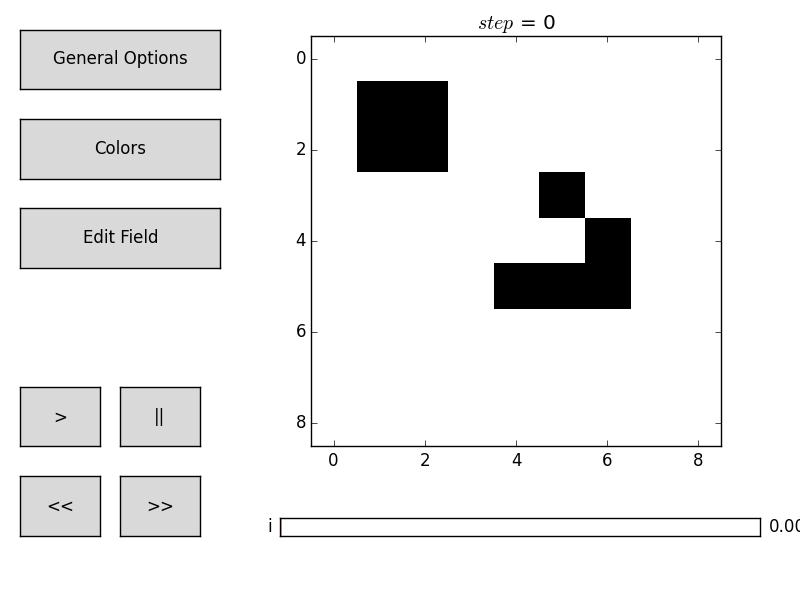
\includegraphics[width=\textwidth]{Gleiter1.png}
		\caption{Anfangsbedingung der Gleiter}
		\label{gleit1}
	\end{center}
\end{figure}
\begin{figure}[p]
	\begin{center}
		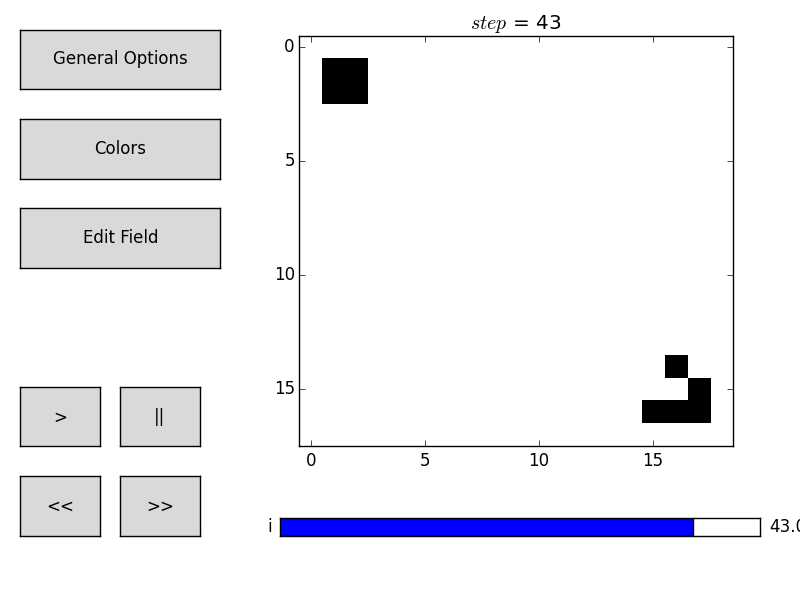
\includegraphics[width=\textwidth]{Gleiter2.png}
		\caption{Felderweiterung durch den Gleiter}
		\label{gleit2}
	\end{center}
\end{figure}

Im Gegensatz dazu verschwindet der Gleiter bei einer endlichen Randbedingung, da er sich nicht weiter bewegen kann. Dieses Beispiel hat die gleiche Anfangsbedingung wie das vorhergehende, ist also ebenfalls unter dem Namen \textit{GameOfLifeGleiter.dat} gespeichert. In Grafik (\ref{gleit3}) erkennt man, wie der Gleiter zu verschwinden beginnt. Ab dem zwölften Schritt wird er zum statischen Quadrat, was in Grafik (\ref{gleit4}) zu erkennen ist.

\begin{figure}[p]
	\begin{center}
		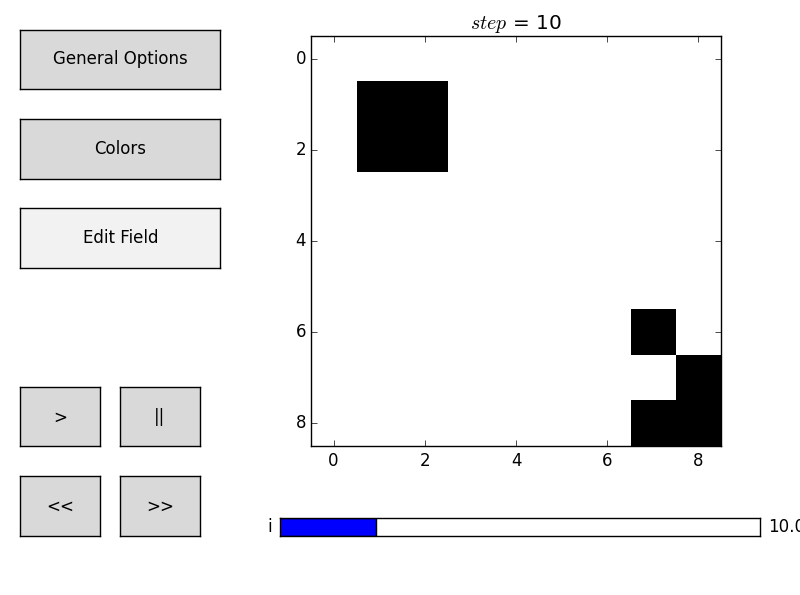
\includegraphics[width=\textwidth]{Gleiter3.png}
		\caption{Gleiter beginnt zu verschwinden}
		\label{gleit3}
	\end{center}
\end{figure}
\begin{figure}[p]
	\begin{center}
		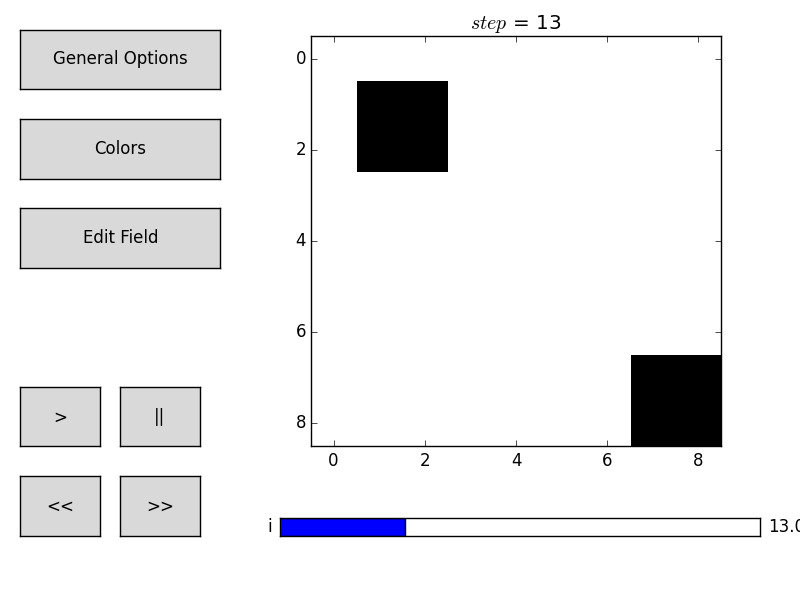
\includegraphics[width=\textwidth]{Gleiter4.png}
		\caption{Gleiter wurde zum Quadrat}
		\label{gleit4}
	\end{center}
\end{figure}

\end{document}